\documentclass[11pt, a4paper]{article}
\usepackage[utf8]{inputenc}
\usepackage{minted}
\usepackage[left=2cm, right=2cm, top=2cm, bottom=1cm, includefoot, headheight=13.6pt]{geometry}
\usepackage[english]{babel}
\usepackage{graphics}
\renewcommand{\baselinestretch}{2.0}

\title{\textbf{Distribute System: Practical Work 1 }}
\vspace{10cm}

\vspace{5cm}
\date{\textbf{January 2022}}
\begin{document}
\maketitle
\begin{enumerate}
  \item BA9-053 Đặng Thái Sơn - Group Leader
  \item BA9-041 Đào Hải Long 
  \item BA9-020 Nguyễn Minh Hiếu
  \item BA9-022 Đỗ Công Hòa
  \item BA9-008 Đoàn Văn Chương
\end{enumerate}
\section{File transfer system}
\hspace{1.5cm}
 Files: \mintinline{text}{send.txt}, \mintinline{text}{receive.txt}
 
\vspace{0.5cm}
I failed to modify provided chat system but I succeed in transferring file with TCP.
\vspace{2cm}

\section{Design Protocol}
\begin{figure}
    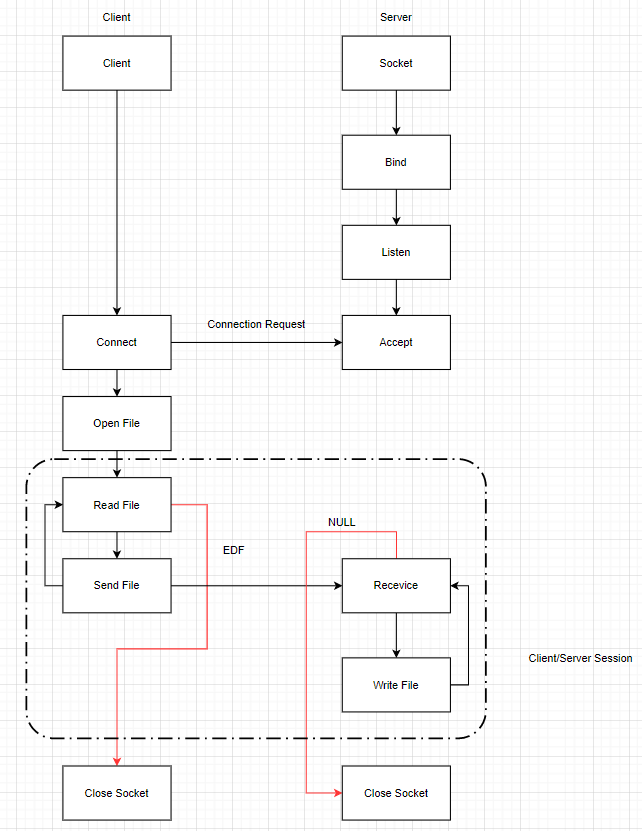
\includegraphics{Image/lab1.png}
    \caption{Protocol}
    \label{fig:my_label}
\end{figure}

\newpage
\section{Organizational system }
\vspace{1cm}
\begin{minted}{text}
                            +--------+
                            | Client |
                            +---+----+
                                |
                                |
                                |
                                | TCP /IP
                                |
                                |
                                v
                            +---+----+
                            | Server |
                            +--------+
\end{minted}
\vspace{0.5cm}
\begin{flushleft}
 The server only listen to one client. The client send data as chunks to the server. After receiving a chunk, the server writes to a file. After finishing writing the file, the server closes itself.
\end{flushleft}
\vspace{0.1cm}

\section{Implementation}
\hspace{0.5cm}
\textbf{ In \mintinline{text}{client_trans.c}, the function to send file is implemented as followed.}
\hspace{1cm}
\begin{minted}{c}

#include <stdio.h>
#include <stdlib.h>
#include <unistd.h>
#include <string.h>
#include <arpa/inet.h>
#define SIZE 1024

void send_file(FILE *fp, int sockfd){
      int n;
      char data[SIZE] = {0};
      while(fgets(data, SIZE, fp) != NULL) {
          if (send(sockfd, data, sizeof(data), 0) == -1) {
             perror("[-]Error in sending file.");
             exit(1);
           }
      bzero(data, SIZE);
     }
  }
 
int main(){
  char *ip = "127.0.0.1";
  int port = 8080;
  int e;
 
  int sockfd;
  struct sockaddr_in server_addr;
  FILE *fp;
  char *filename = "send.txt";
 
  sockfd = socket(AF_INET, SOCK_STREAM, 0);
  if(sockfd < 0) {
    perror("[-]Error in socket");
    exit(1);
  }
  printf("[+]Server socket created successfully.\n");
 
  server_addr.sin_family = AF_INET;
  server_addr.sin_port = port;
  server_addr.sin_addr.s_addr = inet_addr(ip);
 
  e = connect(sockfd, (struct sockaddr*)&server_addr, sizeof(server_addr));
  if(e == -1) {
    perror("[-]Error in socket");
    exit(1);
  }
  printf("[+]Connected to Server.\n");
 
  fp = fopen(filename, "r");
  if (fp == NULL) {
    perror("[-]Error in reading file.");
    exit(1);
  }
 
  send_file(fp, sockfd);
  printf("[+]File data sent successfully.\n");
 
  printf("[+]Closing the connection.\n");
  close(sockfd);
 
  return 0;
}                        
\end{minted}
\vspace{0.5cm}
\hspace{0.5cm}
 \textbf{In \mintinline{text}{server_trans.c}, the function to write file is implemented as followed}
 \hspace{1cm}
\begin{minted}{c}
#include <stdio.h>
#include <stdlib.h>
#include <string.h>
#include <arpa/inet.h>
#define SIZE 2048
 
void write_file(int sockfd){
  int n;
  FILE *fp;
  char *filename = "receive.txt";
  char buffer[SIZE];
 
  fp = fopen(filename, "w");
  while (1) {
    n = recv(sockfd, buffer, SIZE, 0);
    if (n <= 0){
      break;
      return;
    }
    fprintf(fp, "%s", buffer);
    bzero(buffer, SIZE);
  }
  return;
}
 
int main(){
  char *ip = "127.0.0.1";
  int port = 8080;
  int e;
 
  int sockfd, new_sock;
  struct sockaddr_in server_addr, new_addr;
  socklen_t addr_size;
  char buffer[SIZE];
 
  sockfd = socket(AF_INET, SOCK_STREAM, 0);
  if(sockfd < 0) {
    perror("[-]Error in socket");
    exit(1);
  }
  printf("[+]Server socket created successfully.\n");
 
  server_addr.sin_family = AF_INET;
  server_addr.sin_port = port;
  server_addr.sin_addr.s_addr = inet_addr(ip);
 
  e = bind(sockfd, (struct sockaddr*)&server_addr, sizeof(server_addr));
  if(e < 0) {
    perror("[-]Error in bind");
    exit(1);
  }
  printf("[+]Binding successfull.\n");
 
  if(listen(sockfd, 10) == 0){
     printf("[+]Listening....\n");
  }
  else{
    perror("[-]Error in listening");
    exit(1);
 }
  addr_size = sizeof(new_addr);
  new_sock = accept(sockfd, (struct sockaddr*)&new_addr, &addr_size);
  write_file(new_sock);
  printf("[+]Data written in the file successfully.\n");
 
  return 0;
}
\end{minted}

\end{document}
